\section{Model compression with SVD may lose performance quickly}\label{sec:mismatch}

\begin{figure}[b] %[htbp]
   \centering
   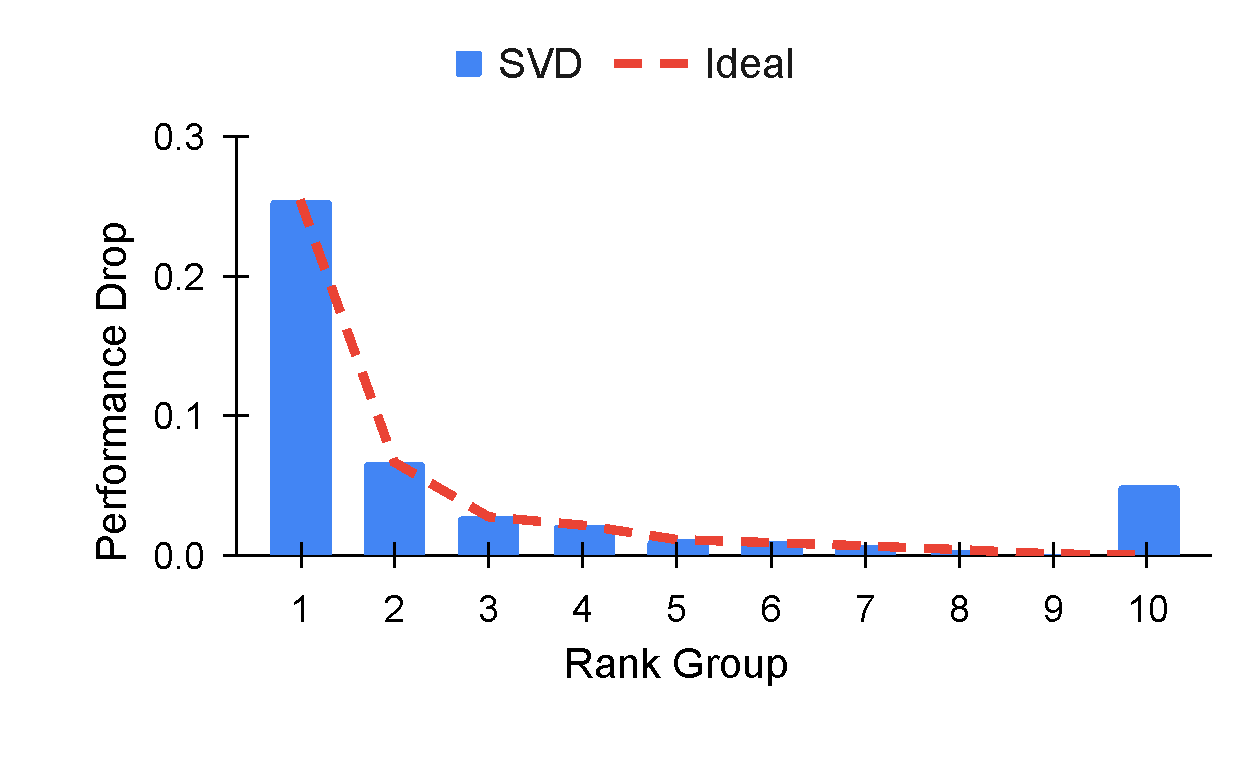
\includegraphics[clip, trim=0cm 1.5cm 0cm 0.8cm,width=0.55\textwidth]{figures/method_fig1_drop.pdf}
       \caption{The grouped truncation and its performance. The truncation of the 10th group, which has the smallest singular values resulting from SVD, is expected to have a minor performance impact (\ie, follow the ideal trend of red dashed line), but this may not be true in actual cases (blue bar).}
       \label{fig:method_rank}
\end{figure}

The singular values in $S$ implicitly give an importance score for a group of parameters. Since the small singular values will be truncated first, those parameters affected by the truncation are expected to be not important for the task performance. We verify the above assumption with a brute force attack: truncate one singular value at a time, then reconstruct the matrix, put it into a model, evaluate and get its performance. Ideally, we hope to see less performance drop when we truncate the smaller singular values. This process can be written as having the reconstructed model weights $\bar W_i$ with the $i$-th singular value be truncated:
\begin{equation}
    \bar W_i = {u_1}{\sigma _1}v_1^T + ... + {u_{i-1}}{\sigma _{i-1}}v_{i-1}^T + {u_{i+1}}{\sigma _{i+1}}v_{i+1}^T + ... + {u_k}{\sigma _k}v_k^T,
    \label{equ:splitting}
\end{equation}
where $u_i$ and $v_i$ are the $i$-th column in $U$ and $V$, correspondingly.

Applying this brute force attack to test a deep neural network is not straightforward since a model can have hundreds of linear layers. Therefore, we truncate a group of singular values together instead of only one. Specifically, we split the singular values of a layer into 10 groups sorted by their values. The 1st group has the top 10\% singular values, while the 10th group contains the smallest 10\% values. When we truncate a specific group, \eg, 5th group, the 5th group of all the layers in a model are truncated together. In other words, we observe the summed impact in a rank group. This results in a smoothed trend for the observation.

Figure \ref{fig:method_rank} plots the result of truncating the 10 groups separately in a standard 12-layer BERT model \citep{devlin2018bert} trained for STS-B task \citep{cer-etal-2017-semeval}. The red dashed line shows an ideal trend which has a smaller performance drop with the tail groups. The blue bars show the actual performance drop. The 10th group surprisingly caused a performance drop as large as the 2nd group. This means the parameters associated with the 10th group are as important as the 2nd group. However, the magnitude of singular value does not reflect this importance, causing a model to lose its performance quickly even when truncating only a small portion.

% As the singular values are in descending order ${\sigma _1} \ge {\sigma _2} \ge  \cdots {\sigma _k} > 0$, the splitting of Equation \ref{equ:splitting} generates rank-pieces ${u_i}{\sigma _i}v_i^T$ of matrix $W$ in order of importance. 
% When conducting low-rank approximation, SVD will first remove the tail rank-pieces, in order to minimize the reconstruction errors.
% Here is a hidden assumption that: lower the reconstruction errors will always reduce the 
% performance drop compared to the original matrix.

% Is that really the case?
% To evaluate this assumption, we split the rank-pieces of SVD into 10 groups, remove one group each time, and calculate the performance drop for each removal correspondingly.
% The results are plotted in Figure \ref{fig:method_rank}.
% Ideally, for any $i<j$, removing rank-piece ${u_i}{\sigma _i}v_i^T$ will cause more performance drop than rank-piece ${u_j}{\sigma _j}v_j^T$, which corresponds to the red line in the figure. 
% However, as shown in the figure,  the tail group of SVD causes more performance drop than most of its preceders.


\begin{figure}%[!b]
  \centering
  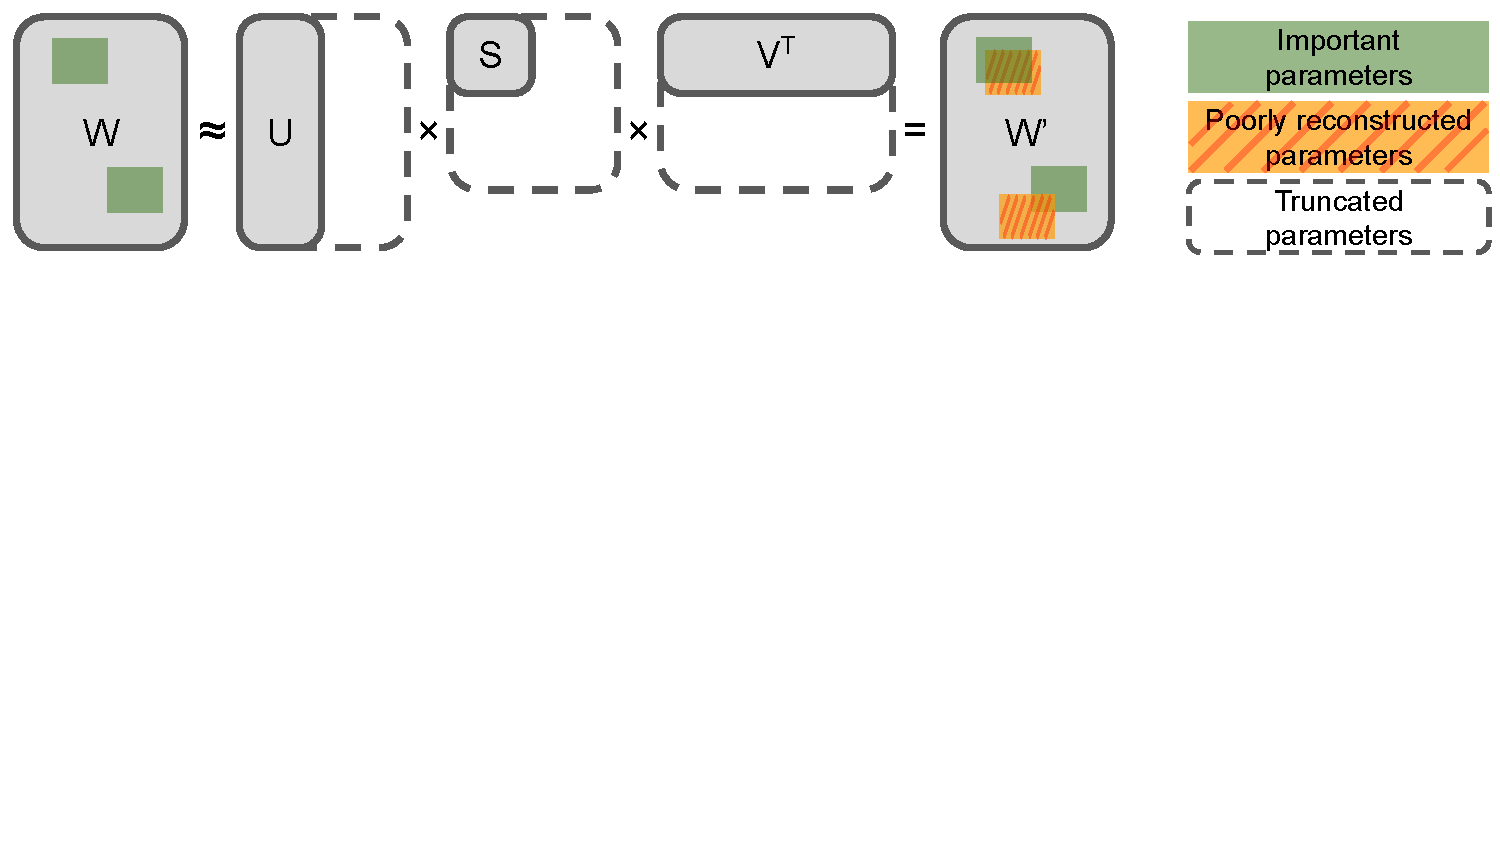
\includegraphics[clip, trim=0cm 9.5cm 0cm 0cm, width=0.75\textwidth]{figures/fig_svd.pdf} 
  \caption{The dilemma of vanilla SVD. Some parameters (the overlap of meshed orange and green) that significantly impact the task performance may not be reconstructed well by SVD because their associated singular values are small and truncated. 
%   Note the reconstruction ($W'$) is shown only for demonstration and is not used to replace the original weights. 
%   Note all the rectangles are 2-D matrices, but we paint only a block for brevity.
  }\label{fig:svd}
\end{figure} 

\begin{figure}%[!b]
  \centering
  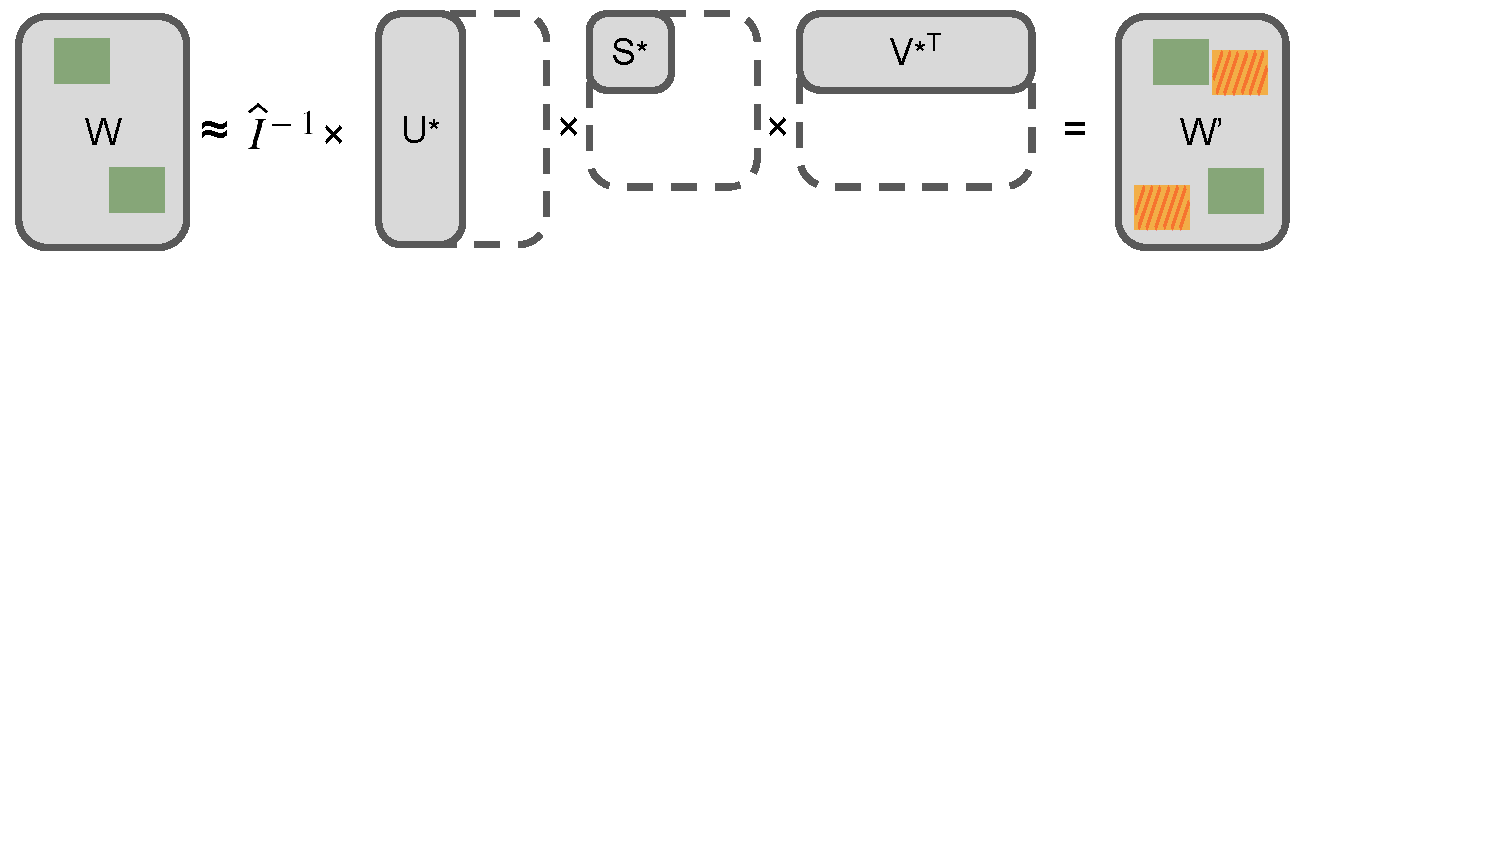
\includegraphics[clip, trim=0cm 9.5cm 3.5cm 0cm, width=0.66\textwidth]{figures/fig_wsvd.pdf} 
  \caption{The schematic effect of our Fisher-Weighted SVD (FWSVD). $\hat I$ is a diagonal matrix containing estimated Fisher information of parameters. By involving Fisher information to weigh the importance, our method reduces the overlap between meshed orange and green, making less performance drop after truncation. 
%   Details are in Section \ref{sec:wsvd}.
  }\label{fig:wsvd}
\end{figure} 

\section{Fisher-weighted low-rank approximation}\label{sec:wsvd}

The issue in Section \ref{sec:mismatch} has an intuitive cause: the optimization objective of SVD does not consider each parameter's impact on the task performance. This issue is illustrated in Figure \ref{fig:svd}, and we address it by introducing the Fisher information into SVD's optimization objective, described as below.

In the generic low-rank approximation, its objective minimizes $||W-AB||_2$. SVD can solve this problem efficiently by having $A=US$ and $B=V^T$. Since we can obtain the importance of each element $W_{ij}$ in $W$, we weigh the individual reconstruction error by multiplying with the estimated Fisher information $\hat {I}_{W_{ij}}$:
% The vanilla SVD is designed to factorize a regular matrix. 
% However, each parameter in the weight matrix of the Transformer has different importance over the loss. 
% In the ideal case, these ``important'' parameters should be remained ``unchanged'' after the compressing of Transformers. 
% To achieve this goal, we replace the original SVD with a novel low-rank approximation weighted by Fisher information. 
% The key idea is to compute the Fisher information for each weight parameter in a trained Transformer and assign this Fisher information value as the weight for low-rank approximation. 
% In this way, the construction process of low-rank approximation will penalize more for modifying ``sensitive'' parameters.
% Give $I(w)$, can be approximated by minimizing
\begin{equation}
\min\limits_{A,B} \sum\limits_{i,j} \hat {I}_{W_{ij}} (W_{ij} - (AB)_{ij})^2.
\label{equ:weight_svd}
\end{equation}
% where $U \in \R^{M \times l}$, $V \in \R^{N \times l}$, and $l$ is the targeted rank.
% ${\hat I}_{{A_{i,j}}}$ is the empirical Fisher information of element $A_{i,j}$.

In general, weighted SVD does not have a closed-form solution \citep{srebro2003weighted} when each element has its weight. To make our method easy to deploy and analyze, we propose a simplification by making the same row of the $W$ matrix to share the same importance. The importance for the row $i$ is defined to be the summation of the row, \ie, $\hat {I}_{W_i}=\sum\limits_{j} \hat {I}_{W_{ij}}$.

% To simplify the problem, we assume that the elements in the same row of the matrix share the same weight. 
Define the diagonal matrix $\hat I= diag(\sqrt{\hat I_{W_1}},...,\sqrt{\hat I_{W_N}})$, then the optimization problem of Equation (\ref{equ:weight_svd}) can be written as:
\begin{equation}
\mathop {\min }\limits_{A,B} ||\hat IW - \hat IAB|{|_2}.
\label{equ:weight_svd_diag}
\end{equation}
Equation \ref{equ:weight_svd_diag} can be solved by the standard SVD on $\hat IW$. We use the notation $svd(\hat IW)=(U^*, S^*, V^*)$, then the solution of Equation (\ref{equ:weight_svd_diag}) will be $A={\hat I}^{ - 1} U^* S^*$, and $B=V^{*T}$. In other words, the solution is the result of removing the information $\hat I$ from the factorized matrices. Figure \ref{fig:wsvd} illustrates this process and its schematic effect of reducing the overlap between important parameters and poorly reconstructed parameters. We will measure this overlap with the performance drop analysis of Section \ref{sec:mismatch}. Lastly, to compress $W$, we will have $A={\hat I}^{ - 1} U_r^* S_r^*$, and $B=V_r^{*T}$, where $r$ denotes the truncated $U^*$, $S^*$, and $V^*$ with reserving only $r$ ranks.  

We call the above method FWSVD in this paper. One thing to highlight is that since we share the same optimization process with the standard SVD, any advantage we observed will be the result of a direct contribution from the $\hat I$ in Equation (\ref{equ:weight_svd_diag}). 
% Moreover, the row-based importance $\hat I$ has an intuitive illustration in Figures \ref{fig:wsvd}, providing a tool to analyze the mismatch between the objectives of low-rank factorization and target task performance.

% We can solve (\ref{equ:weight_svd_diag}) by conducting low-rank approximation of $\hat IA$.
% Assume $(\hat U, \hat S, \hat V)$ is the SVD low-rank solution of $\hat IA$ that $\hat IA \approx \hat U\hat S{{\hat V}^T}$, then the solution of Eqaution (\ref{equ:weight_svd_diag}) will be $U^*={{\hat I}^{ - 1}}\hat U\hat S$, and $V^*=\hat V$.

